\documentclass[12pt,a4paper]{article}
\usepackage{graphicx}
\usepackage{gensymb}
\usepackage{amsmath}
\usepackage{bm}
\usepackage{tikz}
\tikzset{
    node distance=2cm, % specifies the minimum distance between two nodes. Change if necessary.
    }
\title{Case Study Modelling an Electronic Component}
\author{
  Azure Hutchings
  \and
  Jean-Luc Danoy
  \and
  Faris Saad S Alsubaie
}
\date{28 October 2019}
 
\begin{document}
 
\begin{titlepage}
\maketitle
\end{titlepage}

\renewcommand{\abstractname}{Executive Summary}
\begin{abstract}
Write Abstract Here
\end{abstract}

\pagebreak

\tableofcontents

\pagebreak

\section{Introduction}

\subsection{Purpose of the Report}
The following report investigates the steady-state heat distribution in a newly designed component. 

The report will discuss the mathematical model of the heat distribution in the component and the numerical methods used to solve it in MATLAB. 

\subsection{The Maths of the Problem}

\begin{figure}[h!]
	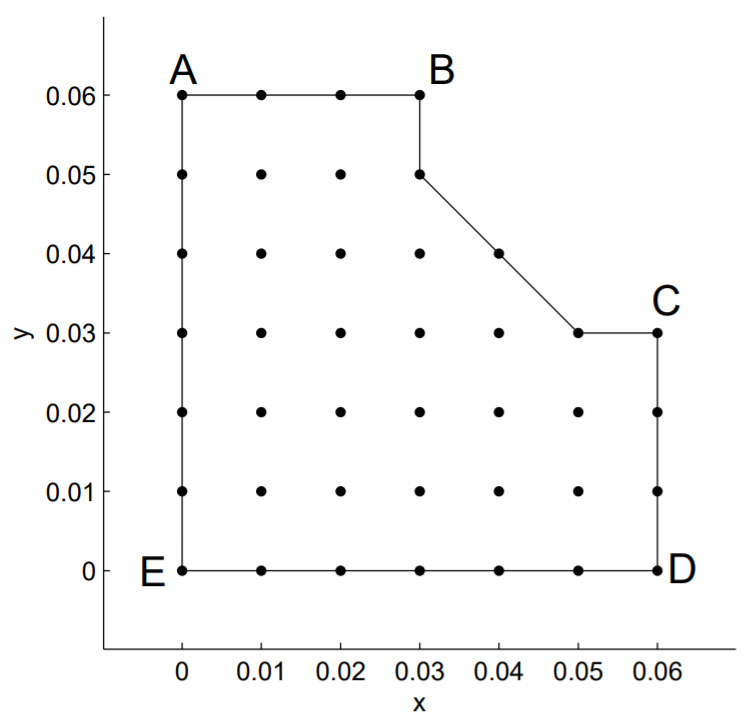
\includegraphics[width=\linewidth]{images/Component.png}
	\caption{Schematic of electronic component.}
	\label{fig:componentSchematic}
\end{figure}

The component schematic is shown in Figure \ref{fig:componentSchematic}. The location of the component within the device means it's subject to different temperature condition along it's boundaries. The boundary A-B is in perfect thermal contact with another component which the temperature is known to 70\degree C. The boundary C-D is also in perfect thermal contact with another component which the temperature is known to be 40\degree C. The boundary A-E-D is thermally insulated and the boundary B-C is exposed to the air at ambient temperature.
\\\\
This type of model can be described with Laplace's equation. Letting $T(x,y)$ represent the temperature of the component at point $(x, y)$, the model is as follows	

\begin{center}
\begin{tabular}{c c}
$\frac{\partial^2 T}{\partial x^2}+\frac{\partial^2 T}{\partial y^2}=0$ & in the interior\\
$T = 70$ & on boundary A-B \\
$T = 40$ & on boundary C-D \\
$\boldsymbol{\nabla} T \cdot {\hat{\textbf{n}}} = 0$ & on boundary A-E-D\\
$k\boldsymbol{\nabla}T\cdot\hat{\textbf{n}} = h(T_{\infty} - T)$ & on boundary B-C
\end{tabular}
\end{center}
Where the thermal conductivity is $k=3Wm^{-1}C^{-1}$, and the heat transfer coefficient is $h=20 Wm^{-2}C^{-1}$. To begin with, we will assume the ambient termperature is $T_\infty = 20$.
\clearpage

